\documentclass[12pt,letter]{article}
\usepackage{../downey_format}




\begin{document}
	
	% set the section number, along with figure and equation numbers
	\setcounter{section}{4}	
	\setcounter{figure}{0}   
	\renewcommand\thefigure{\thesection.\arabic{figure}}
	\setcounter{equation}{0}   
	\renewcommand\theequation{\thesection.\arabic{equation}}
	\section{Decision Trees}


Decision trees are flexible learners that work well for classification, regression, and multi-output problems. A single tree can capture intricate relationships in the data with minimal preprocessing. Each tree also acts as the core building block of ensemble methods such as Random Forests, which are among the most reliable models in modern practice. One limitation is size: a fully grown tree can become quite large, so pruning or depth limits are often applied to control memory use and reduce overfitting.

In this chapter, we will explore the essentials of Decision Trees, starting with their training, visualization, and prediction processes. We will then look into the CART (Classification and Regression Trees) training algorithm, which Scikit-Learn utilizes for constructing Decision Trees. Additionally, we will examine how to regulate the complexity of Decision Trees and adapt them for regression tasks. The chapter concludes by addressing some inherent limitations of Decision Trees. 

\begin{figure}[H]
	\centering
	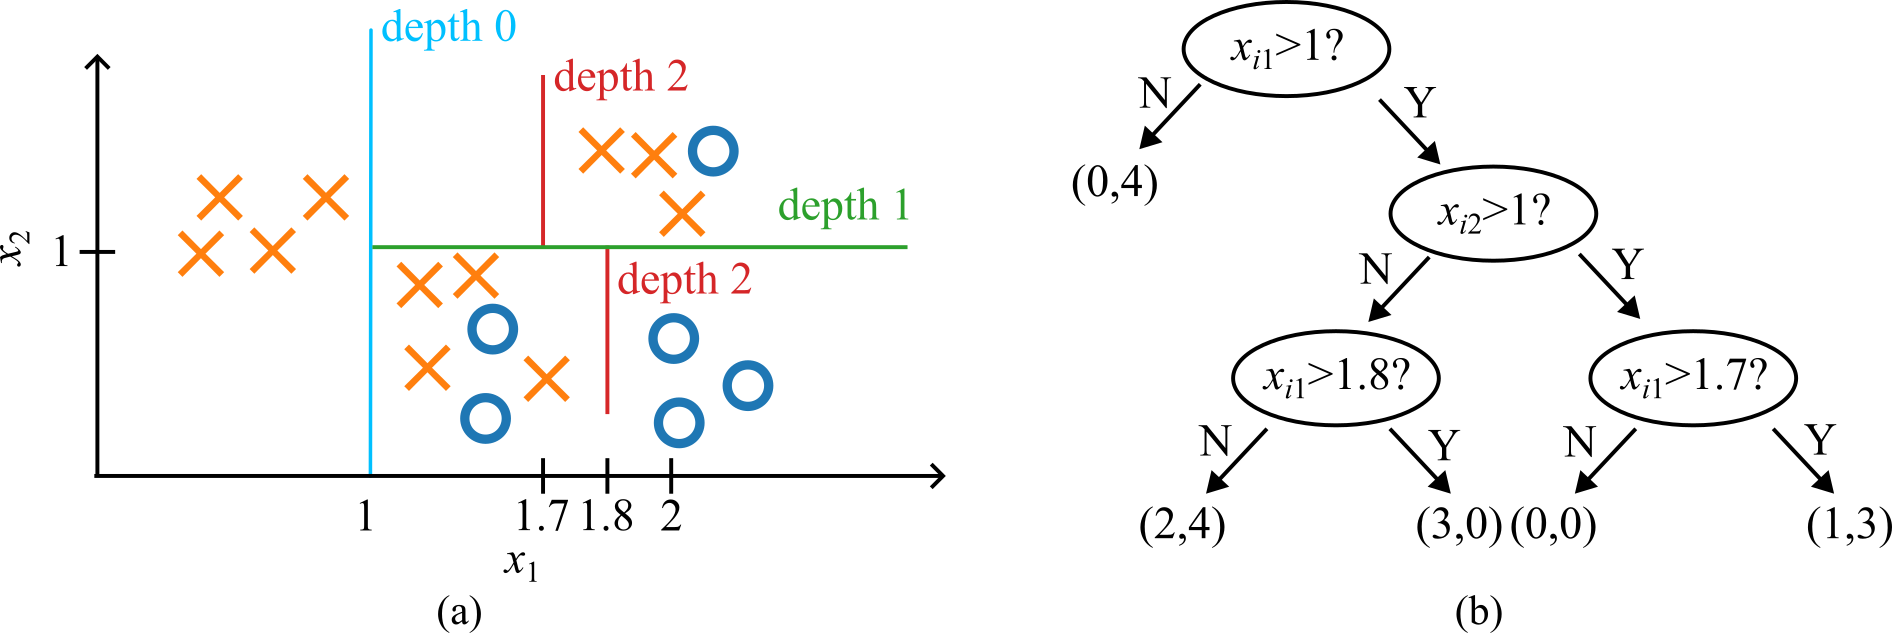
\includegraphics[width=6.5in]{../figures/decision_tree_basic_concept}
	\caption{The basic connect of a decision tree, showing (a)~how a decision tree is built, and (b)~the developed decision tree.}
	\label{fig:decision_tree_basic_concent}
\end{figure}


\subsection{Decision Tree Classification}


Figure~\ref{fig:decision_tree_boundaries} shows the regions formed by the decision tree. The solid vertical line marks the root split at depth�0, where petal length equals 2.45~cm. All samples on the left of this line belong solely to Iris~setosa, so no further division is needed there. The right half still mixes species, so the depth-1 right child splits again at petal width 1.75~cm, indicated by the dashed line. With \texttt{max\_depth}=2 the tree stops at this point. If \texttt{max\_depth} were increased to�3, the two depth-2 leaves would introduce additional boundaries, drawn as dotted lines.


\begin{figure}[H]
	\centering
	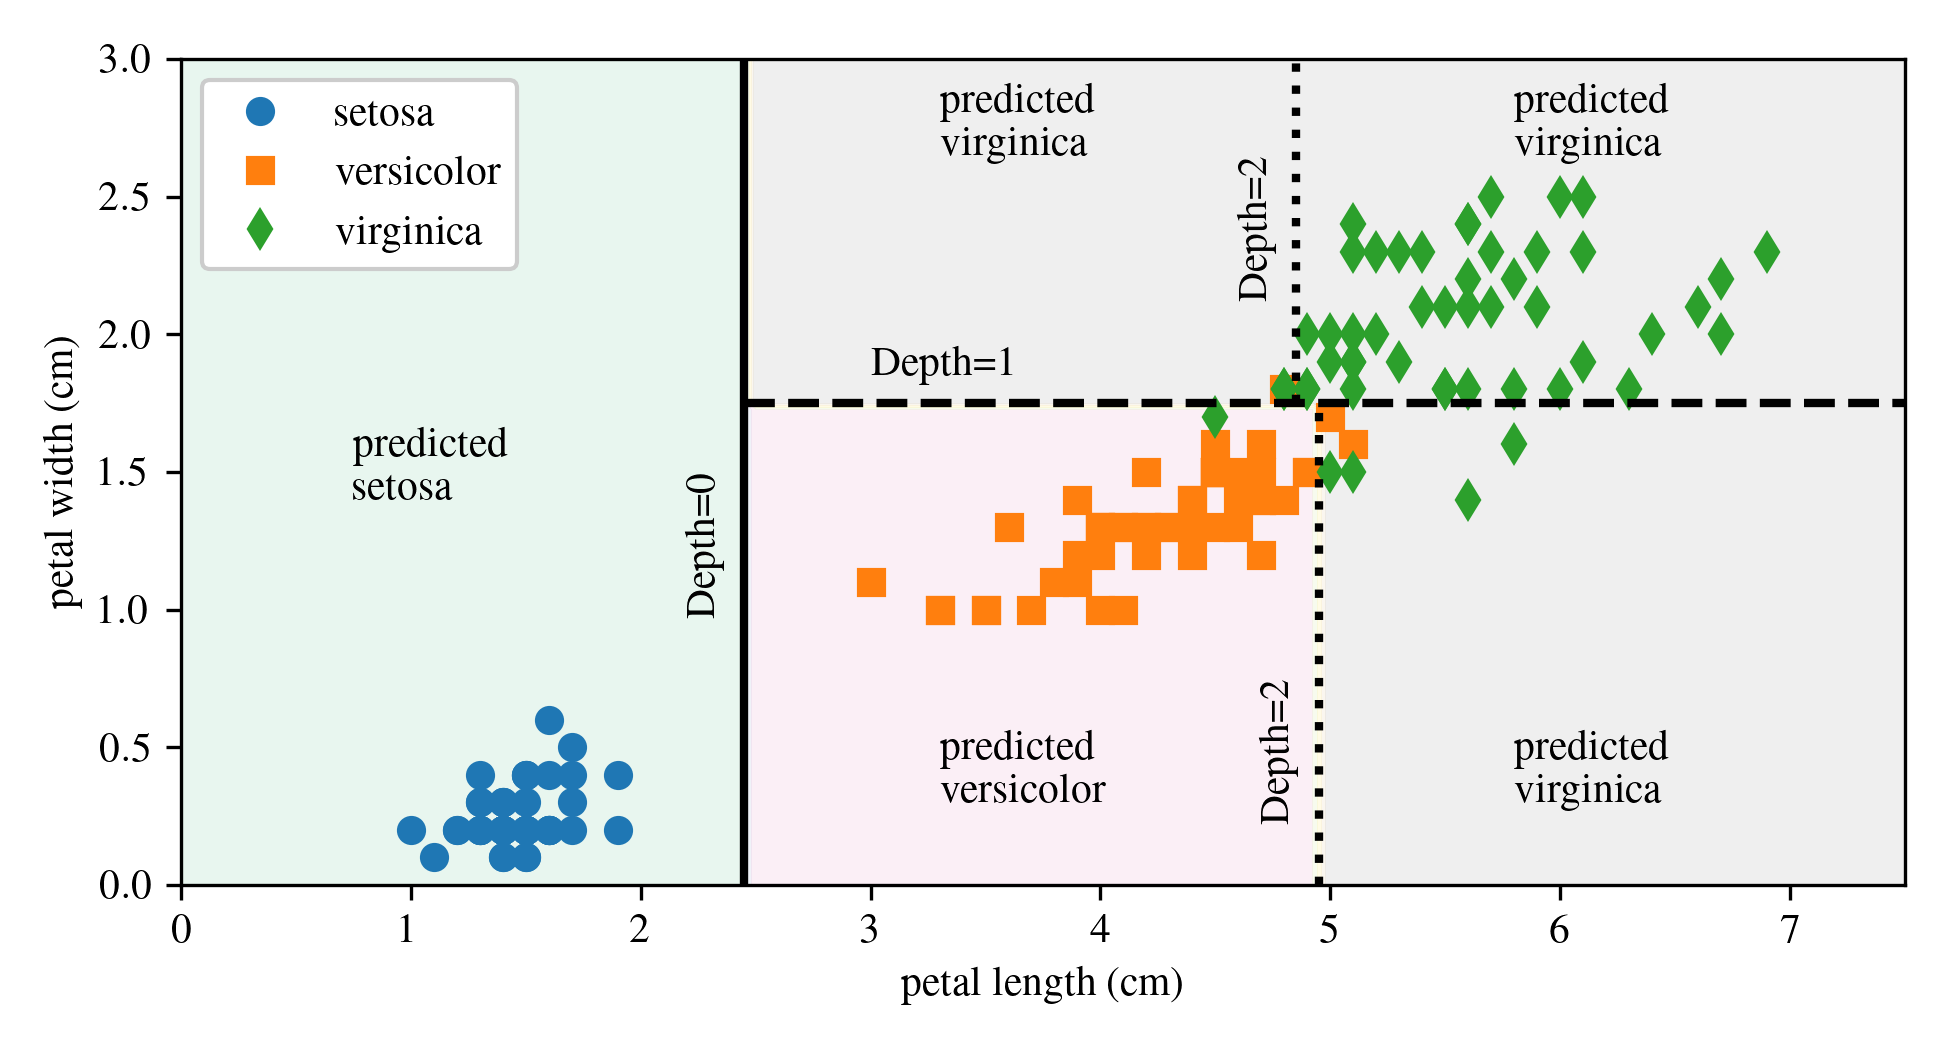
\includegraphics[width=6.5in]{../figures/decision_tree_boundaries}
	\caption{Decision Tree decision boundaries.}
	\label{fig:decision_tree_boundaries}
\end{figure}



A decision tree for the Iris Dataset looks like Figure~\ref{fig:Iris_decision_tree}. Let us examine how the Decision Tree processes predictions. Suppose you come across an iris and need to classify it. Start at the root node (depth=0), which asks whether the flower's petal length is less than 2.45~cm. If the answer is yes, move to the root's left child (depth=1). This child is a leaf, so no further questions follow. The class stored in that leaf is Iris-setosa, and the tree therefore labels the sample as setosa.

\begin{figure}[H]
	\centering
	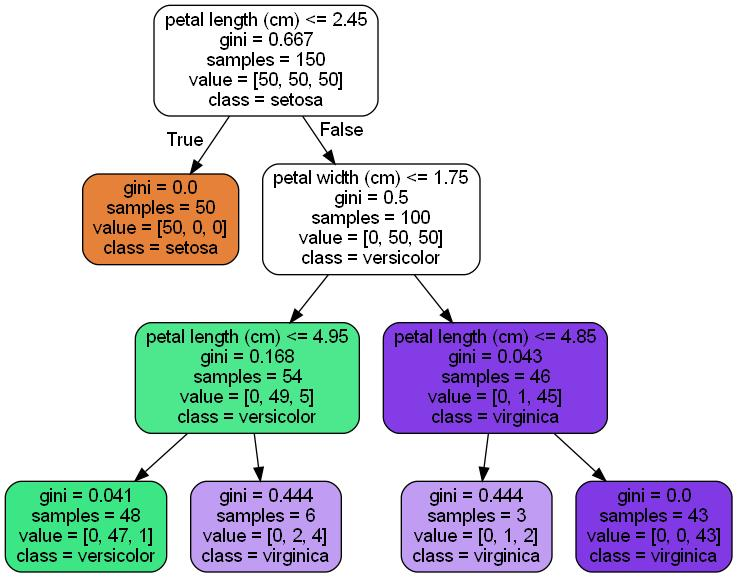
\includegraphics[width=3.5in]{../figures/Iris_decision_tree}
	\caption{Decision tree for the Iris Dataset trained using the CART algorithms.}
	\label{fig:Iris_decision_tree}
\end{figure}

In Figure~\ref{fig:Iris_decision_tree}, each node reports the split criterion, Gini impurity, sample count, and class distribution. Fill colors denote the predicted species; orange for Setosa, green for Versicolor, and purple for Virginica. Shade intensity conveys confidence: darker hues indicate purer (more certain) leaves, whereas white represents complete uncertainty.
Consider a second iris whose petal length is greater than 2.45~cm. From the root you move to its right child (depth~1). This internal node asks a new question: is the petal width less than 1.75~cm? If yes, the flower is classified as Iris-versicolor (depth=2, left leaf). If no, it is labeled Iris-virginica (depth=2, right leaf). The decision path is clear and easy to follow.

The attributes of a node include:
\begin{itemize}
\item \textit{class}: the class label stored in the leaf.
\item \textit{samples}: the number of training instances that reach the node. For example, $100$ flowers have petal length $>$2.45~cm (depth1, right); among them, $54$ also have petal width $<1.75$~cm (depth2, left).
\item \textit{value}: a three-element vector giving the count of instances from each species at the node. The bottom-right leaf, for instance, contains $0$ Iris-setosa, $1$ Iris-versicolor, and $45$ Iris-virginica.
\item \textit{gini}: the Gini impurity. A node is \emph{pure} when $\textit{gini}=0$, meaning all samples belong to the same class. The depth-1 left node, which holds only Iris-setosa, is pure.
\end{itemize}

The Gini impurity $G_i$ for the $i^{th}$ node is computed using
\begin{equation}
	\label{eq:gini_impurity}
	G_i = 1 - \sum_{k=1}^{n}p_{i,k}^2,
\end{equation}
where $p_{i,k}$ is the proportion of class $k$ instances among the training instances at the $i^{th}$ node. For instance, the Gini score for the depth-2 left node is calculated as follows: $1 - (0/54)^2 - (49/54)^2 - (5/54)^2 \approx 0.168$. We will discuss an alternative impurity measure later.





\subsubsection{Class Probability Estimation}

A Decision Tree can estimate the likelihood that a sample belongs to class~$k$. The algorithm traces the sample's path to its leaf node and then reports the fraction of training instances of class~$k$ found in that leaf. Consider a flower with petals 5cm long and 1.5cm wide. This sample reaches the depth-2 left leaf, which contains 54 training flowers: 0 \textit{Iris}-setosa, 49 \textit{Iris}-versicolor, and 5 \textit{Iris}-virginica. The tree therefore assigns probabilities of 0\%, 90.7\%, and 9.3\% to the three classes, respectively. When asked for a class label, it selects \textit{Iris}-versicolor, the class with the highest probability.

Interestingly, the same estimated probabilities apply throughout the bottom-right rectangle of Figure~\ref{fig:decision_tree_boundaries}, even in a scenario where the petal dimensions are 6~cm by 1.5~cm where one might intuitively expect an Iris-Virginica classification.

\begin{example}
\textbf{Decision Tree Classifier}

\noindent This example uses Scikit-Learn's \texttt{DecisionTreeClassifier} to classify iris species based on petal features. The decision process is visualized using Graphviz, showing the structure of learned rules and how decisions are made based on feature thresholds.  This online viewer is the easiest way to do that \url{https://dreampuf.github.io/GraphvizOnline/}
\end{example}


\subsection{The CART Training Algorithm}

Scikit-Learn trains decision trees with the Classification and Regression Tree (CART) algorithm\footnotemark[1], a process often called ``growing'' the tree. At each node the algorithm splits the local training set into two parts by selecting a feature $k$ and a threshold $t_{k}$, for example ``petal length $\leq 2.45$~cm''. It evaluates every candidate pair $(k,t_{k})$ and chooses the one that yields the purest child nodes, judging purity by a weighted combination of each child's impurity measure and sample count.


\footnotetext[1]{Breiman, Leo. Classification and regression trees. Routledge, 2017}


\begin{figure}[H]
	\centering
	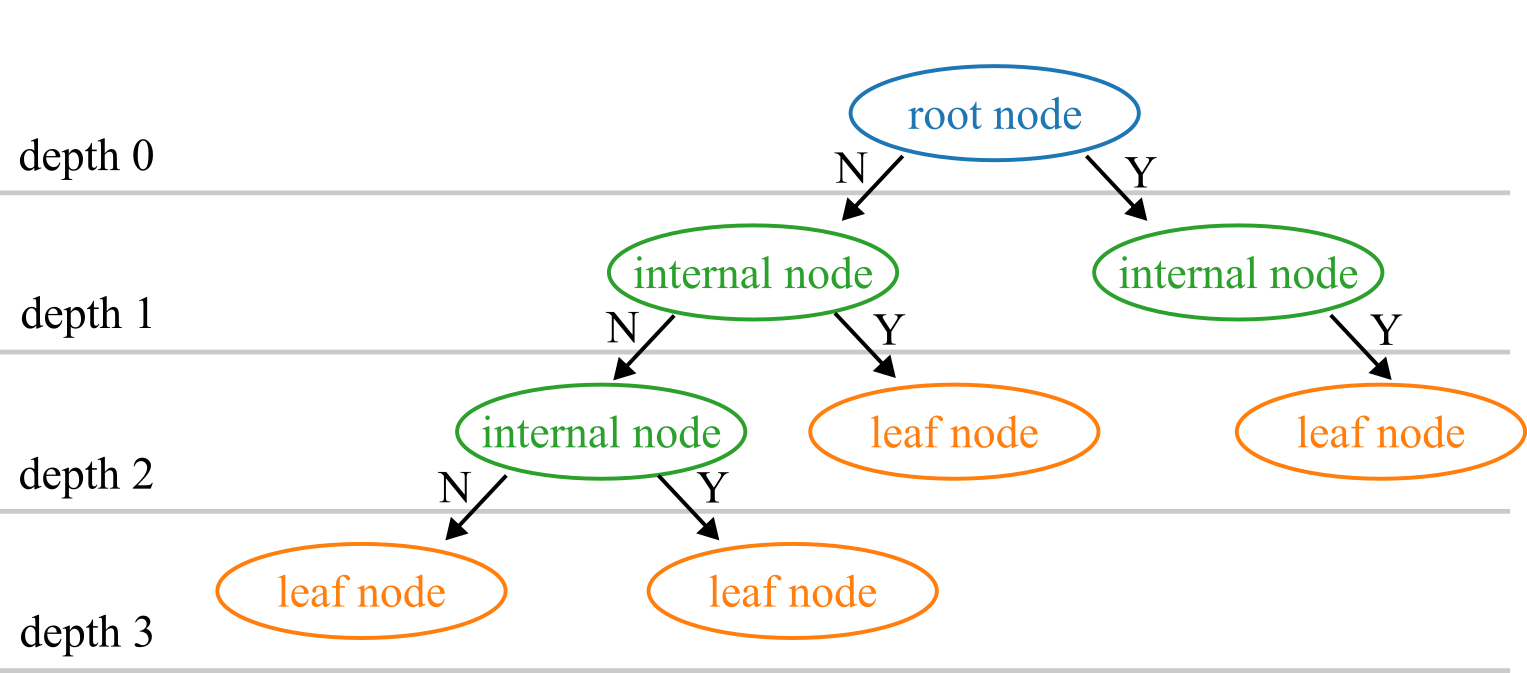
\includegraphics[]{../figures/CART_algorithm}
	\caption{Illustration of the CART algorithm process.}
	\label{fig:algorithm}
\end{figure}


The objective function it aims to minimize during this process is

\begin{equation}
\label{eq:CART_algorithm}
J(k, t_k) = \frac{m_{\text{left}}}{m} G_{\text{left}} + \frac{m_{\text{right}}}{m} G_{\text{right}}. 
\end{equation}

\noindent In this equation, $G_{\text{left}/\text{right}}$ measures the impurity of the left/right subset, and $m_{\text{left}/\text{right}}$ is the number of instances in the left/right subset.
 After the initial split, the algorithm continues to divide the resulting subsets and their subsequent divisions recursively. This recursive process halts when it reaches the predefined maximum depth ({\tt{max\_depth}}) set through a hyperparameter, or if no further impurity-reducing splits can be found.

Unlike linear models that assume a specific data structure, Decision Trees impose few assumptions on their initial data. If not appropriately constrained, a Decision Tree can intricately conform to the training data, leading to overfitting. This model type is described as nonparametric, not due to a lack of parameters, which it can have in abundance, but because the parameters are not predetermined before training, allowing the model's structure to freely mirror the data intricacies. Conversely, a parametric model, like a linear model, has a fixed number of parameters, limiting its flexibility but also minimizing overfitting risks while potentially increasing underfitting risks.

To mitigate overfitting in Decision Trees, it is essential to control the model's freedom during training through regularization. The regularization hyperparameters vary by the algorithm, but typically, the tree's maximum depth can be restricted. In Scikit-Learn, this is managed by the \texttt{max\_depth} hyperparameter, which is unlimited by default. Lowering \texttt{max\_depth} helps regularize the model, thereby reducing overfitting likelihood.

Other parameters in Scikit-Learn's DecisionTreeClassifier also influence the tree's structure:
\begin{itemize}
    \item \texttt{min\_samples\_split}: The minimum number of samples required to split a node.
    \item \texttt{min\_samples\_leaf}: The minimum number of samples a leaf node must have.
    \item \texttt{min\_weight\_fraction\_leaf}: Similar to \texttt{min\_samples\_leaf}, but expressed as a fraction of total weighted instances.
    \item \texttt{max\_leaf\_nodes}: The maximum number of leaf nodes.
    \item \texttt{max\_features}: The maximum number of features evaluated for splitting at each node.
\end{itemize}
Adjusting these parameters by increasing \texttt{min\_}* values or decreasing \texttt{max\_}* values will help regularize the model.

Figure~\ref{fig:decision_tree_regularization} illustrates two Decision Trees trained on the moons dataset: one on the left with default hyperparameters (unrestricted) and another on the right with \texttt{min\_samples\_leaf}=4. The left model appears to be overfitting, whereas the right model, with its restrictions, likely offers better generalization.

\begin{figure}[H]
    \centering
    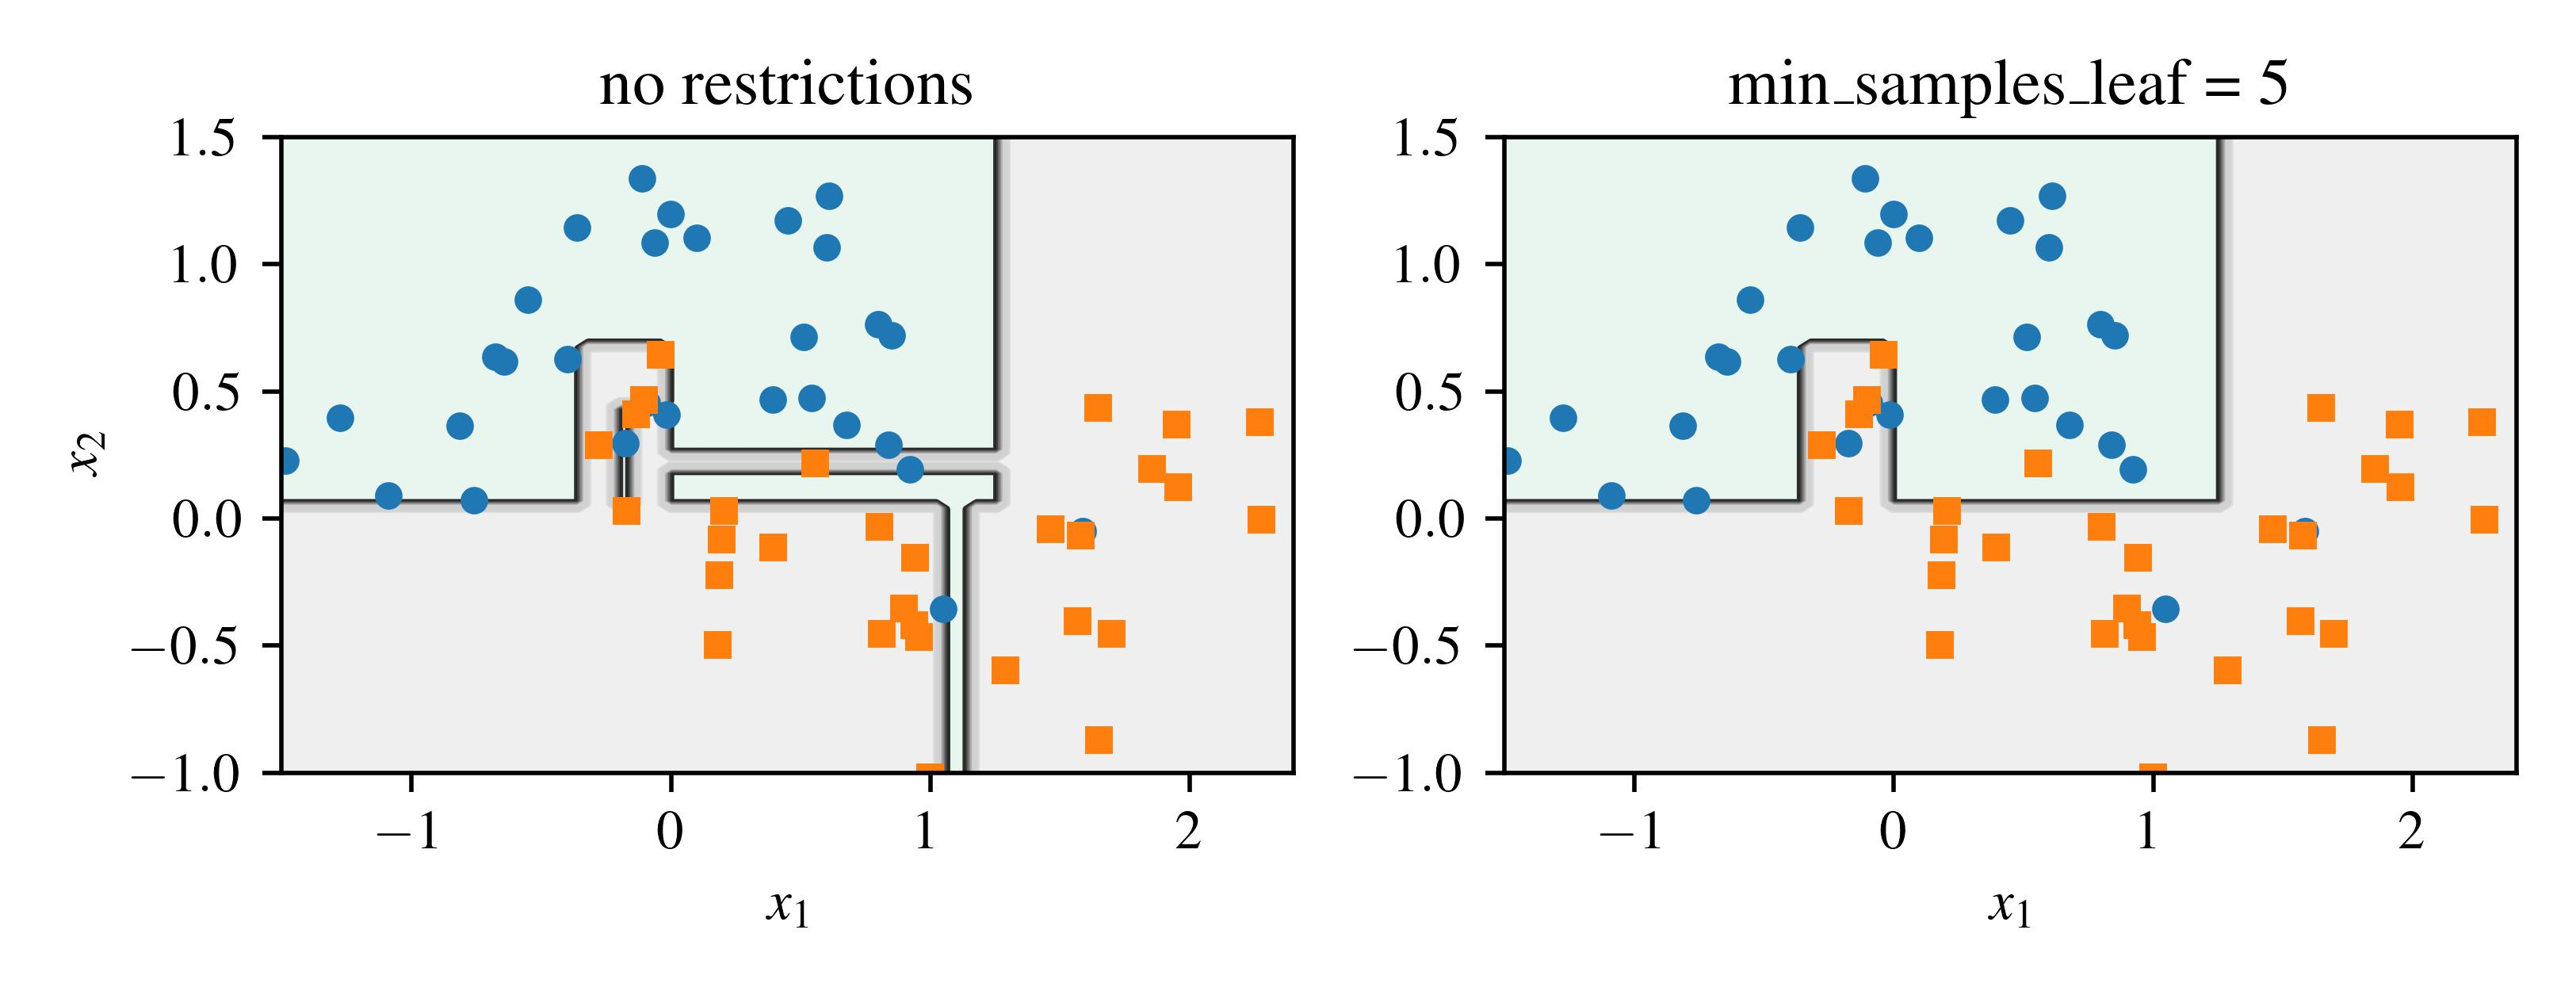
\includegraphics[width=6.5in]{../figures/decision_tree_regularization}
    \caption{Regularization effects using \texttt{min\_samples\_leaf}}
    \label{fig:decision_tree_regularization}
\end{figure}



\subsubsection{Computational Complexity}

To predict with a Decision Tree the algorithm follows a path from the root to a leaf. Because most trained trees are roughly balanced, this path crosses about
\begin{equation}
T_{\text{predict}} = O \bigl(\log_2 m\bigr),
\label{eq:dt_pred_complexity}
\end{equation}
nodes, where $m$ is the number of training samples. Each node tests a single feature, so the prediction cost in equation~\ref{eq:dt_pred_complexity} is unaffected by the total feature count and is therefore very fast.

Training is costlier. At every split the algorithm scans each candidate feature (or the subset limited by \texttt{max\_features}) over all samples that reach the node. For $n$ input features the total work across all levels is
\begin{equation}
T_{\text{train}} = O \bigl(n \times m \log m\bigr),
\label{eq:dt_train_complexity}
\end{equation}
because the tree has roughly $\log_2 m$ layers and each layer processes a shrinking fraction of the $m$ samples.

When the dataset contains only a few thousand samples, enabling \texttt{presort=True} in Scikit-Learn can shorten training time, but for larger datasets the presorting step turns into a bottleneck and the standard (unsorted) approach is quicker.

\subsubsection{Entropy verse Gini Impurity}

Decision Trees in sklearn use the Gini impurity as the default criterion for node purity, entropy can also be utilized by setting the criterion hyperparameter to ``entropy''. Originally a thermodynamic concept representing molecular disorder, entropy reaches zero when molecules are in a complete state of rest and order. This concept was later adopted in information theory, introduced by Shannon, to quantify the average informational content in messages entropy is zero when all messages are identical. In the realm of Machine Learning, entropy serves as a measure of impurity: it is zero in a dataset if all its elements belong to a single class. The entropy for the i\textsuperscript{th} node is defined as


\begin{equation}
	\label{eq:entropy}
    H_i = - \sum_{\substack{k=1 \\ p_{i,k} \neq 0}}^{n} p_{i,k} \log_{2}(p_{i,k}).
\end{equation}

The choice between Gini impurity and entropy often results in negligible differences, producing similar trees. Gini impurity has a slight computational advantage and is thus the default choice. However, it tends to separate the most frequent class into a distinct branch, whereas entropy generally yields more balanced trees.







\subsection{Decision Tree Regression}

Decision Trees are not limited to classification tasks; they can also be adapted for regression. To illustrate, we use Scikit-Learn's \texttt{DecisionTreeRegressor} to train a regression tree on a noisy linear dataset with \texttt{max\_depth}=2. The structure of this tree is displayed in Figure~\ref{fig:decision_tree_regression}. In contract to the color scheme for classification, the change in color shades here relate to the predicted value of $y$.

\begin{figure}[H]
	\centering
	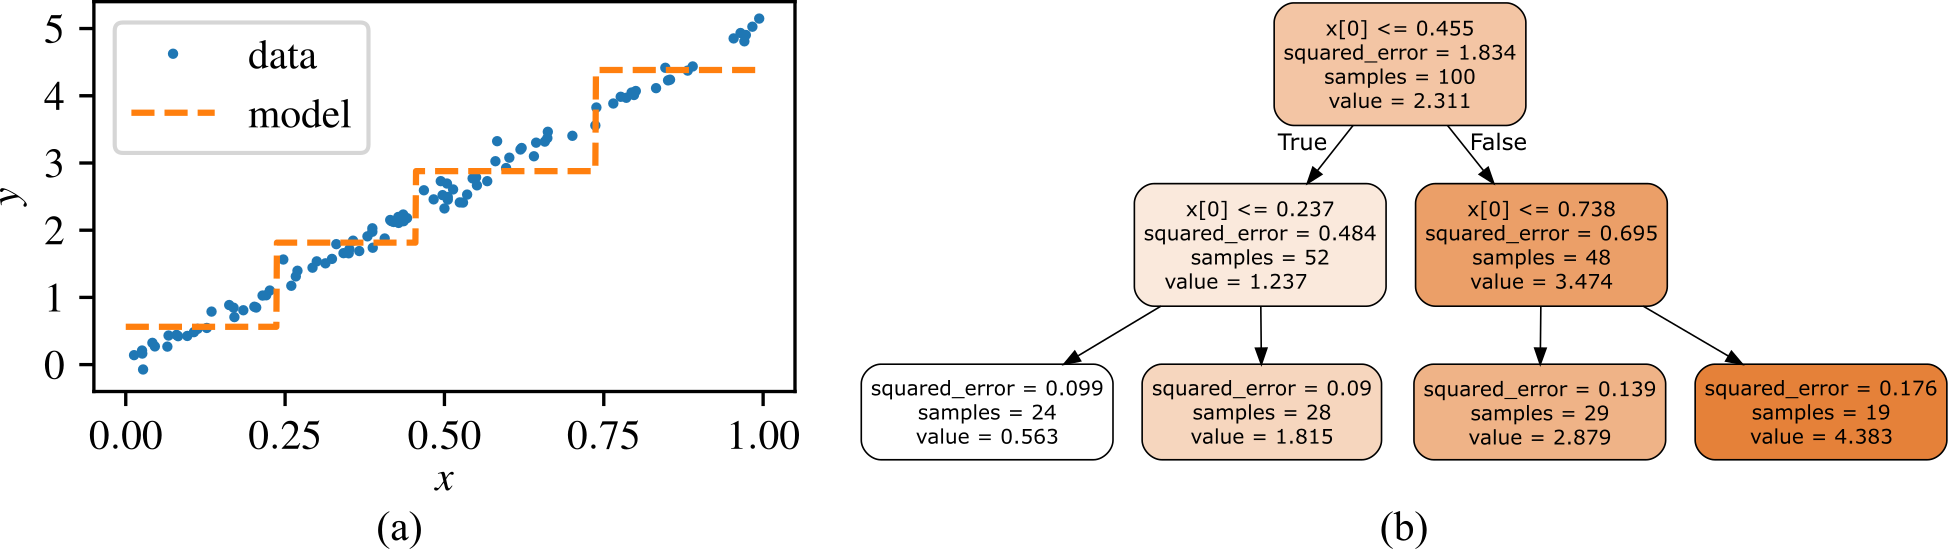
\includegraphics[width=6.5in]{../figures/decision_tree_regression}
	\caption{A regression model developed using a Decision Tree, showing the: (a) model superimposed over noisy data, and (b) the decision tree developed for the task.}
	\label{fig:decision_tree_regression}
\end{figure}

The workings of a regression tree mirror those of a classification tree, except that each leaf holds a continuous prediction instead of a class label. To obtain a prediction for a sample with $x_1 = 0.6$, trace the path from the root to its leaf; that leaf outputs $0.1106$, which is the average target value among the 110 training instances that reach it. For those instances the mean squared error is $0.0151$.

The predictions from this model are visualized in Figure~\ref{fig:decision_tree_regression_prediction}, with results shown for trees of depth 2 and 3. The deeper tree partitions the input space into more regions, with each region's predicted value being the average target value of the instances it encompasses. The model attempts to organize the regions such that the instances within each are as close as possible to their predicted value.

\begin{figure}[H]
	\centering
	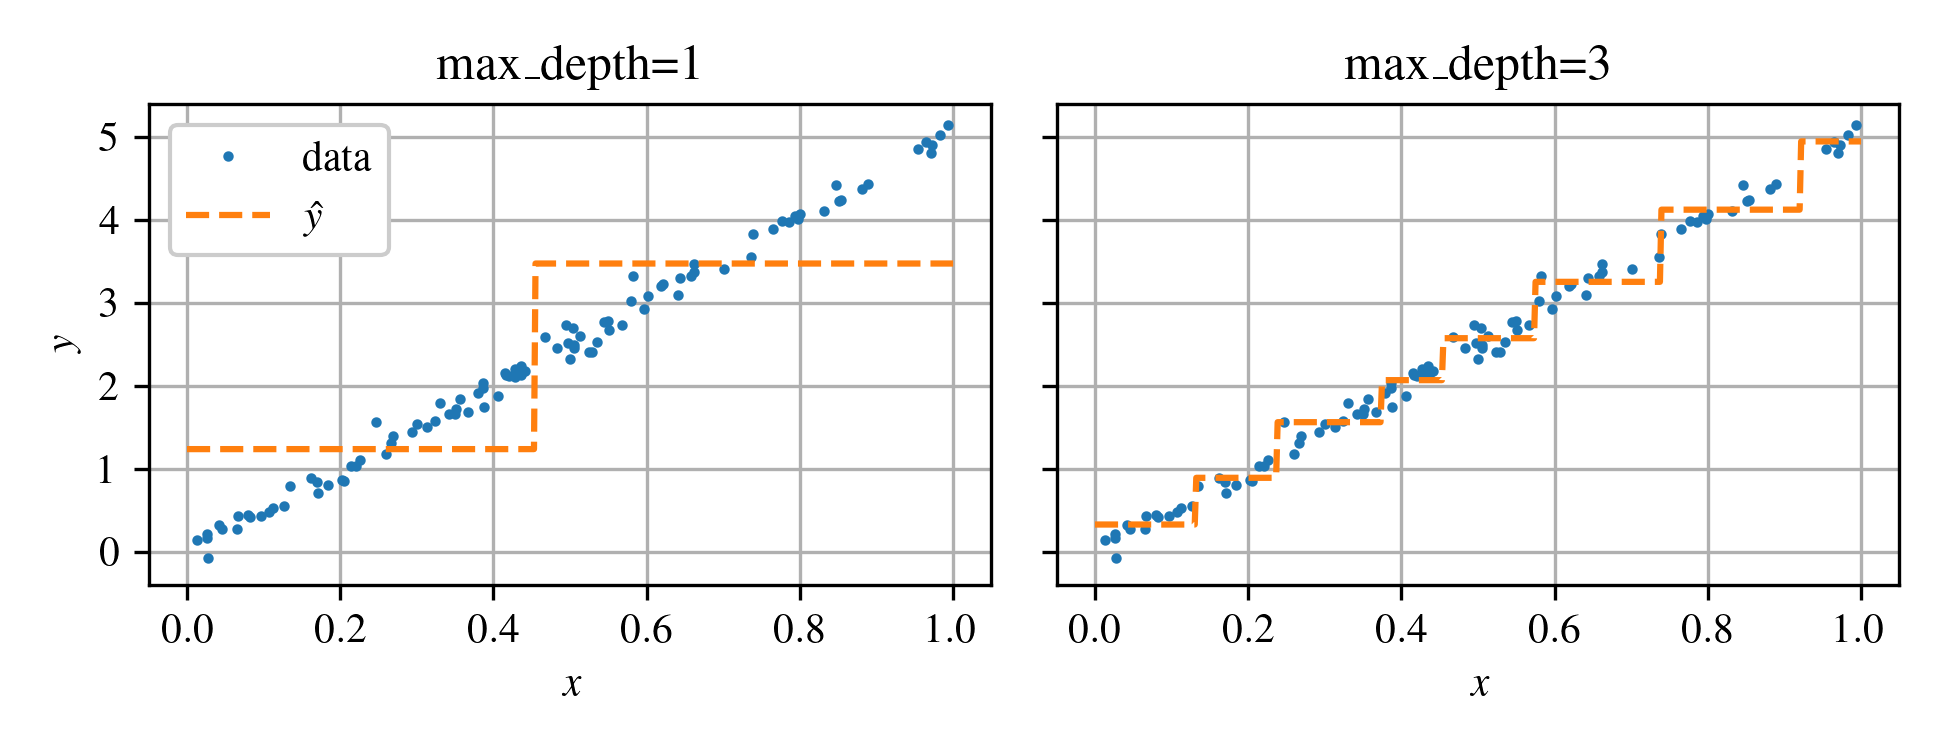
\includegraphics[width=6.5in]{../figures/decision_tree_regression_prediction}
	\caption{Comparison of predictions from two Decision Tree regression models with varying depths.}
	\label{fig:decision_tree_regression_prediction}
\end{figure}

The CART algorithm for regression trees aims to minimize the MSE when splitting the training set, similar to how it minimizes impurity in classification tasks. The cost function minimized by the algorithm is represented as

\begin{equation}
	\label{eq:CART_regression}
    J(k, t_k) = \frac{m_{\text{left}}}{m} \text{MSE}_{\text{left}} + \frac{m_{\text{right}}}{m} \text{MSE}_{\text{right}}.
\end{equation}
Knowing that, 
\begin{equation}
	\text{MSE}_{\text{node}} = \sum\limits_{i \in \text{node}} \left( \hat{y}_{\text{node}} - y^{(i)} \right)^2
\end{equation}
and
\begin{equation}
\hat{y}_{\text{node}} = \frac{1}{m_{\text{node}}} \sum\limits_{i \in \text{node}} y^{(i)}.
\end{equation}

% \quad \text{where} \quad 
%    \left\{
%    \begin{array}{l}
%         \\
%        \hat{y}_{\text{node}} = \frac{1}{m_{\text{node}}} \sum\limits_{i \in \text{node}} y^{(i)}
%    \end{array}
%    \right.
%\end{equation}

Similar to classification, Decision Trees for regression can overfit if not properly regularized. Without regularization, the predictions, as depicted on the left of Figure~\ref{fig:decision_tree_regression_regularized}, can fit the training data excessively. By setting \texttt{min\_samples\_leaf} to 15, a more generalized model is achieved, as shown on the right in the same figure.

\begin{figure}[H]
	\centering
	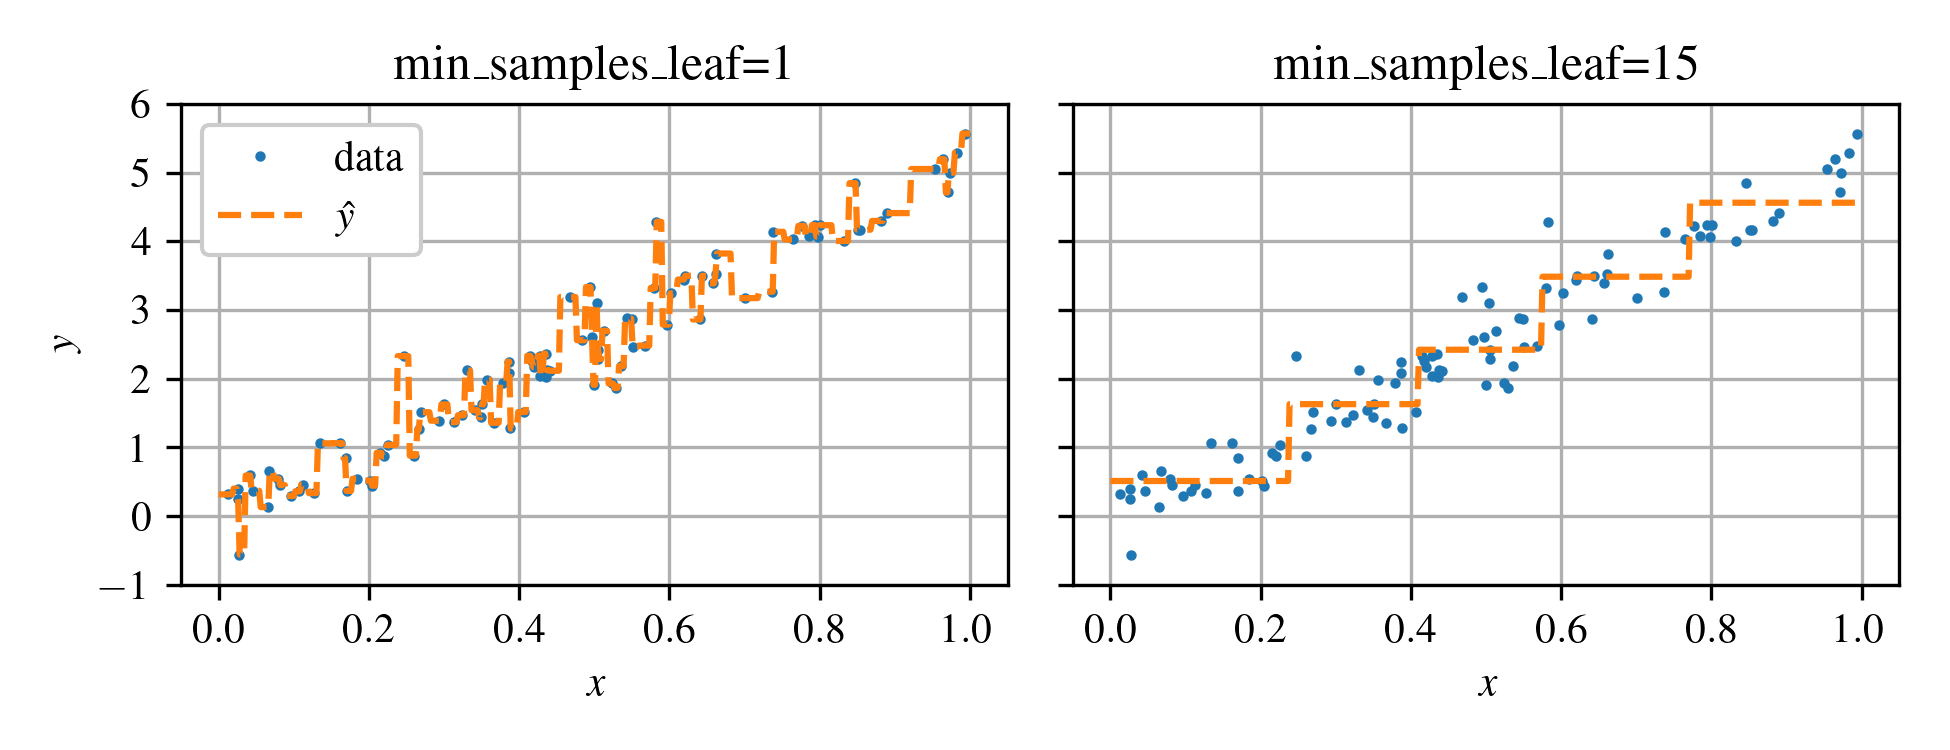
\includegraphics[width=6.5in]{../figures/decision_tree_regression_regularized}
	\caption{Impact of regularization through setting the minimum number of samples in a leaf on a Decision Tree regression model.}
	\label{fig:decision_tree_regression_regularized}
\end{figure}


\begin{example}
\textbf{Decision Tree Regression}

\noindent This example uses Scikit-Learn's \texttt{DecisionTreeRegressor} to fit a non-linear relationship between input and output data. A tree of depth 4 is trained on noisy linear data and visualized using Graphviz to show how the regression model partitions the input space.
\end{example}



\subsection{Instability}

While Decision Trees offer simplicity, interpretability, versatility, and power, they come with certain drawbacks. A notable limitation is their preference for orthogonal decision boundaries, which makes them highly sensitive to the orientation of the data. For instance, Figure~\ref{fig:decision_tree_training_rotation} illustrates how a simple linearly separable dataset can be perfectly split by a Decision Tree in its original alignment, whereas a 45� rotation results in a convoluted decision boundary. Despite perfect fits to their respective training sets, the rotated tree's model is likely to perform poorly on unseen data. Utilizing Principal Component Analysis (PCA) can often mitigate this issue by reorienting the data more suitably.

\begin{figure}[H]
	\centering
	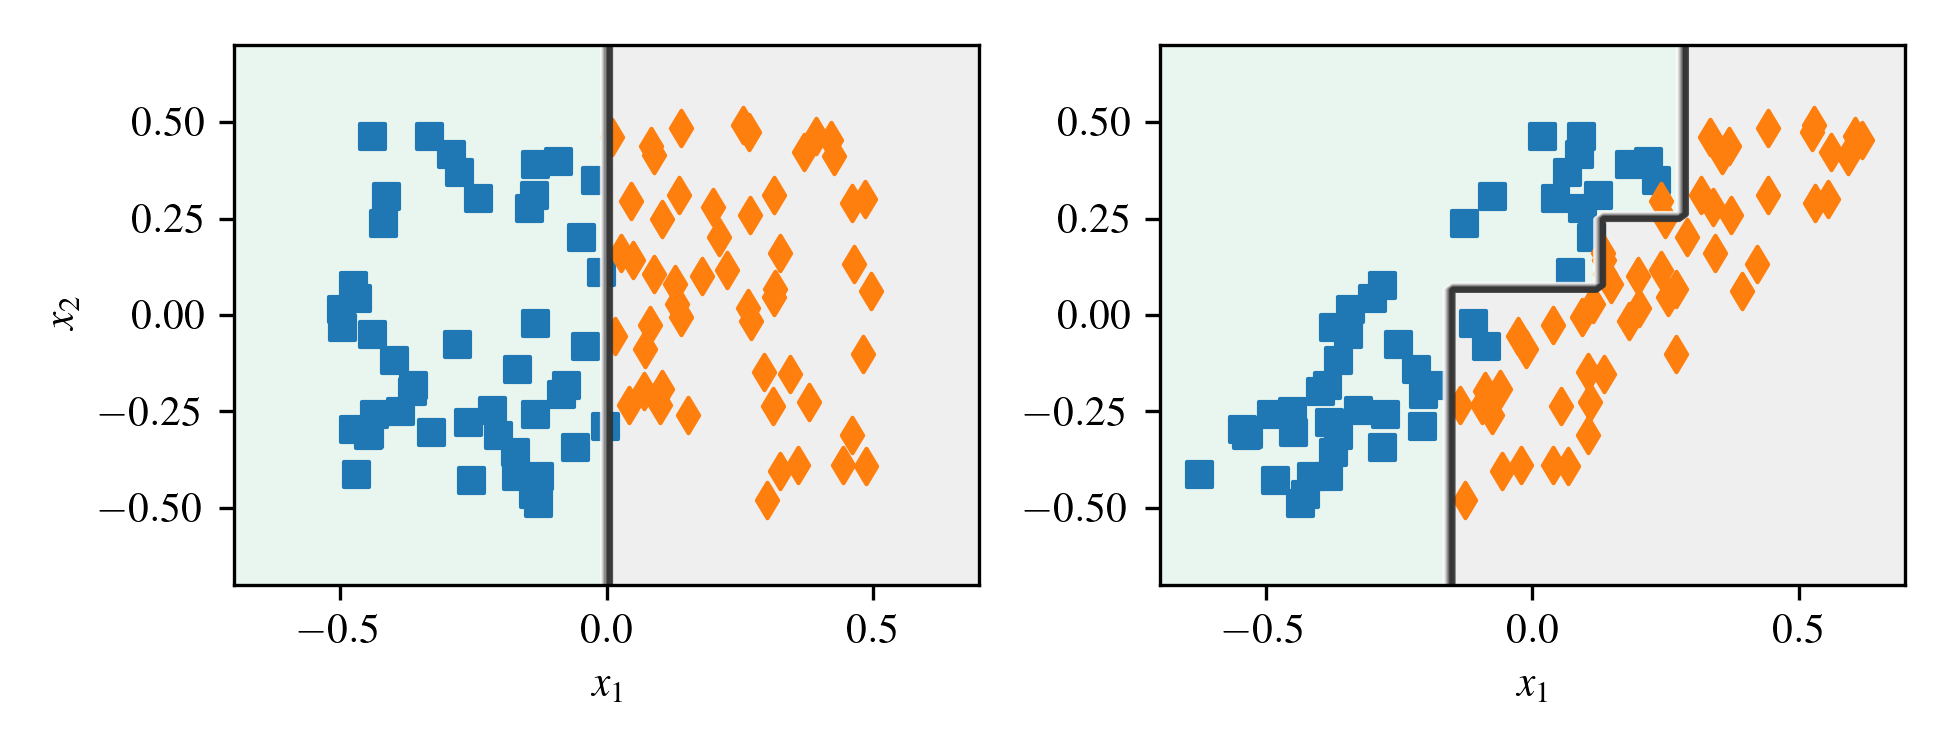
\includegraphics[width=5.5in]{../figures/decision_tree_training_rotation}
	\caption{Sensitivity to training set rotation. Decision trees create a single clean split on the original data (left), but after a $45^\circ$  rotation they must build a jagged, multi-step boundary; illustrating their sensitivity to feature orientation.}
	\label{fig:decision_tree_training_rotation}
\end{figure}

More broadly, Decision Trees are sensitive to small variations in training data. For instance, changing the seed of the random number generator can lead to a substantially different model, as shown in Figure~\ref{fig:decision_tree_training_details_1}. This variability is partly due to the stochastic nature of the Scikit-Learn's training algorithms; different models may result from the same data unless the \texttt{random\_state} hyperparameter is fixed.

\begin{figure}[H]
	\centering
	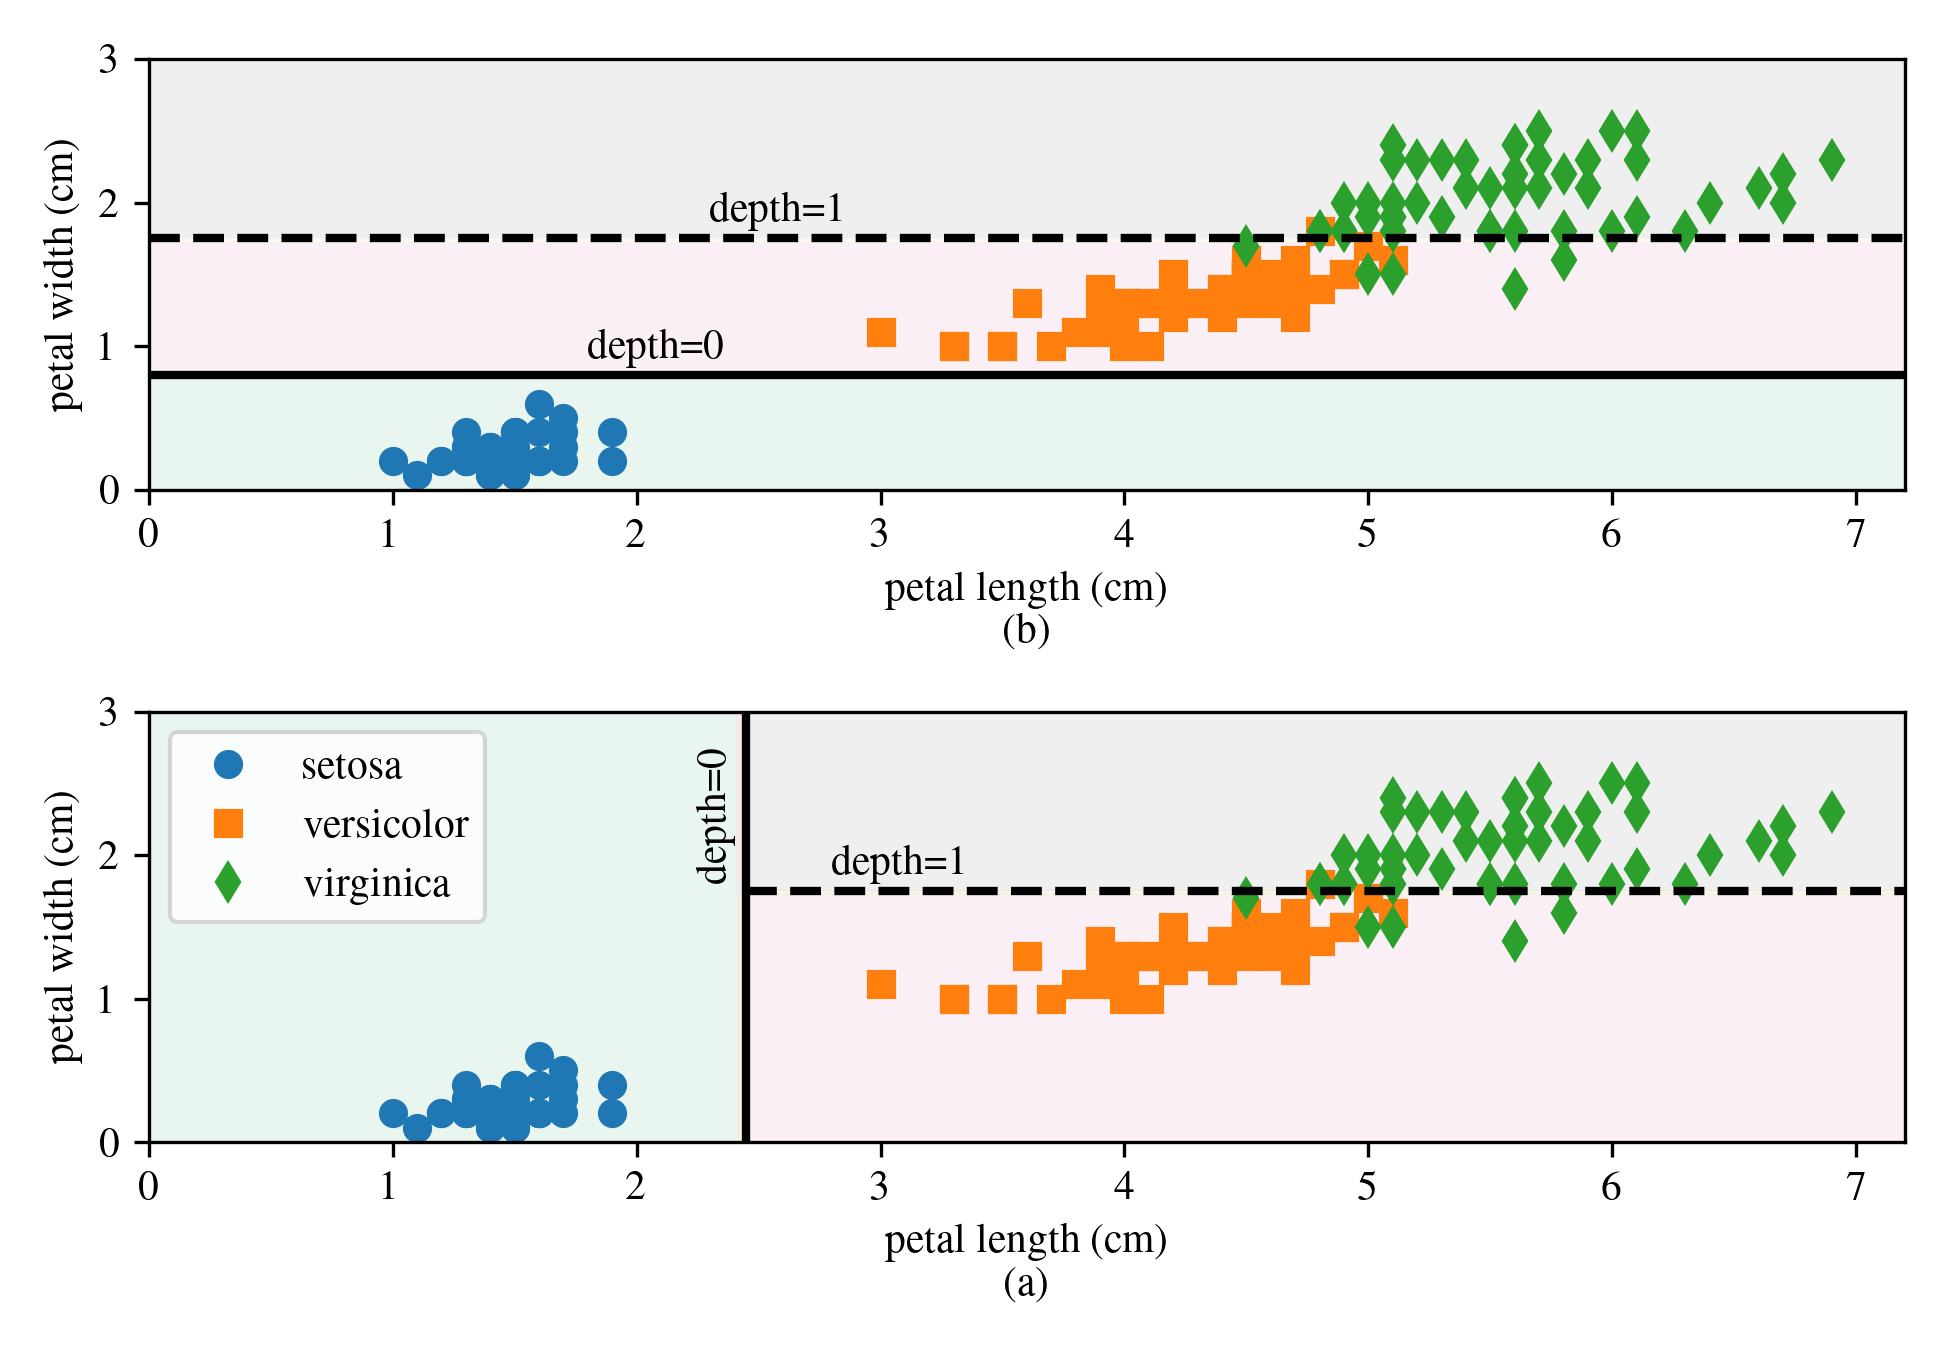
\includegraphics[width=6.0in]{../figures/decision_tree_sensitivity}
	\caption{Decision Tree Sensitivity to initial conditions, showing: (a) random number generator seeded with ``1'', and: (b) random number generator seeded with ``2''. \protect\footnotemark[1] }
	\label{fig:decision_tree_training_details_1}
\end{figure}


\footnotetext[1]{``2'' is the author's preferred random number seed.}



\subsection{Random Forest}
\begin{figure}[H]
	\centering
	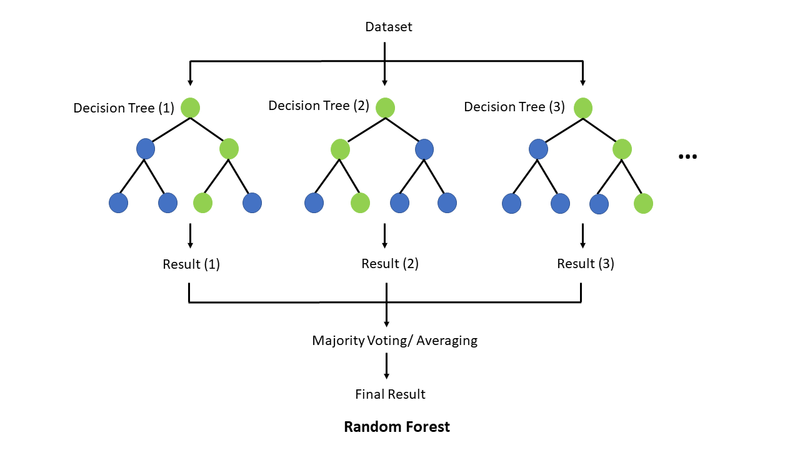
\includegraphics[width=6.5in]{../figures/random_forest}
	\caption{Random forest with majority voting. \protect\footnotemark[1]} 
	\label{fig:random_forest}
\end{figure}

\footnotetext[1]{TseKiChun, CC BY-SA 4.0 $<$https://creativecommons.org/licenses/by-sa/4.0$>$, via Wikimedia Commons}


Random Forests reduce the high variance of individual decision trees by building many trees on bootstrap samples of the training data and then averaging their outputs. Each tree is grown with a random subset of input features, so the ensemble decorrelates the trees and improves generalisation. For classification problems the forest predicts the class that receives the majority vote, while for regression it returns the mean of the trees' numeric predictions. This bagging strategy limits overfitting and usually yields better performance than a single tree, although it often falls short of the accuracy achieved by gradient-boosted ensembles. Model quality still depends on the data's size, noise level, and feature interactions, and on hyperparameters such as the number of trees, the maximum depth, and the number of features considered at each split.

\pagebreak
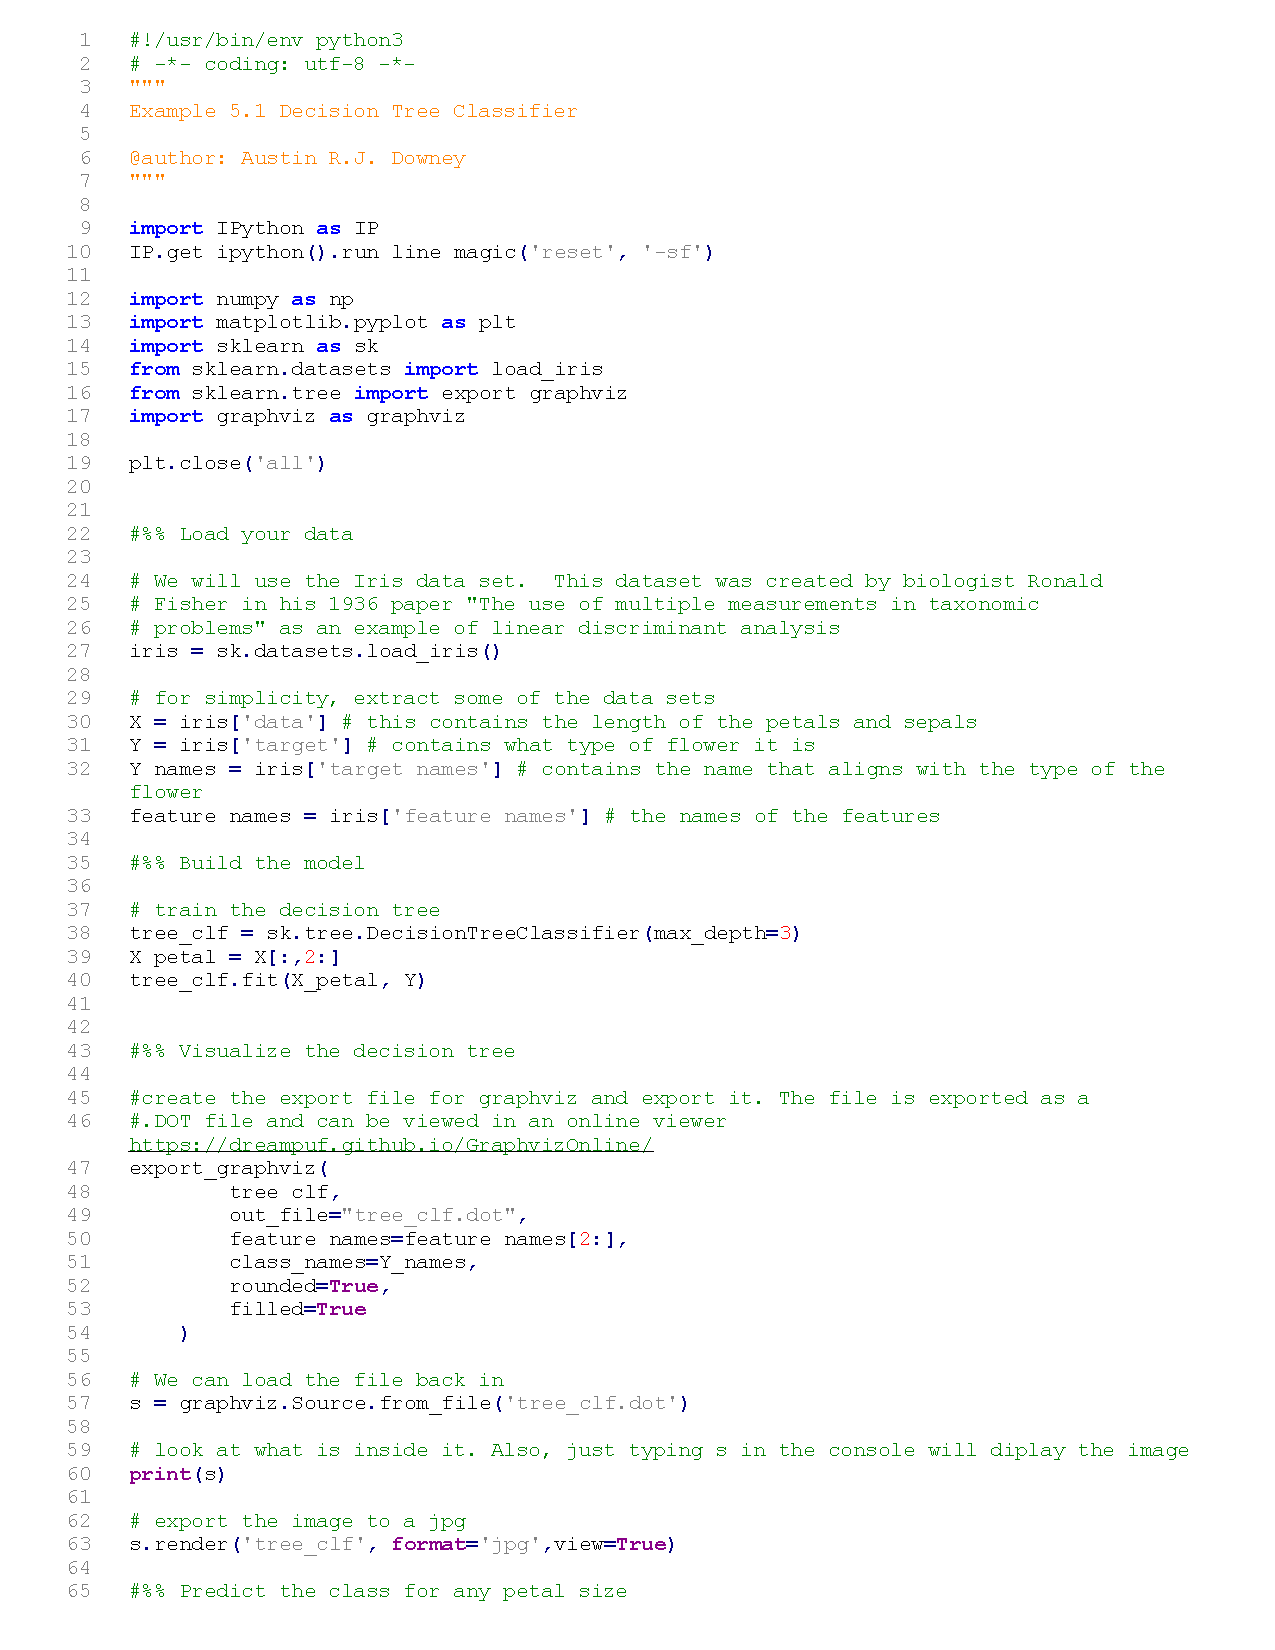
\includepdf[pages=1, width= 0.95\textwidth, pagecommand = {\subsection{Examples} \subsubsection*{Example 5.1}\vspace{0.5em}}]{../code/example_5.1_DecisionTree_Classifier.pdf}
\includepdf[pages=2, width= 0.95\textwidth, pagecommand = {\vspace{0.5em}}]{../code/example_5.1_DecisionTree_Classifier.pdf}

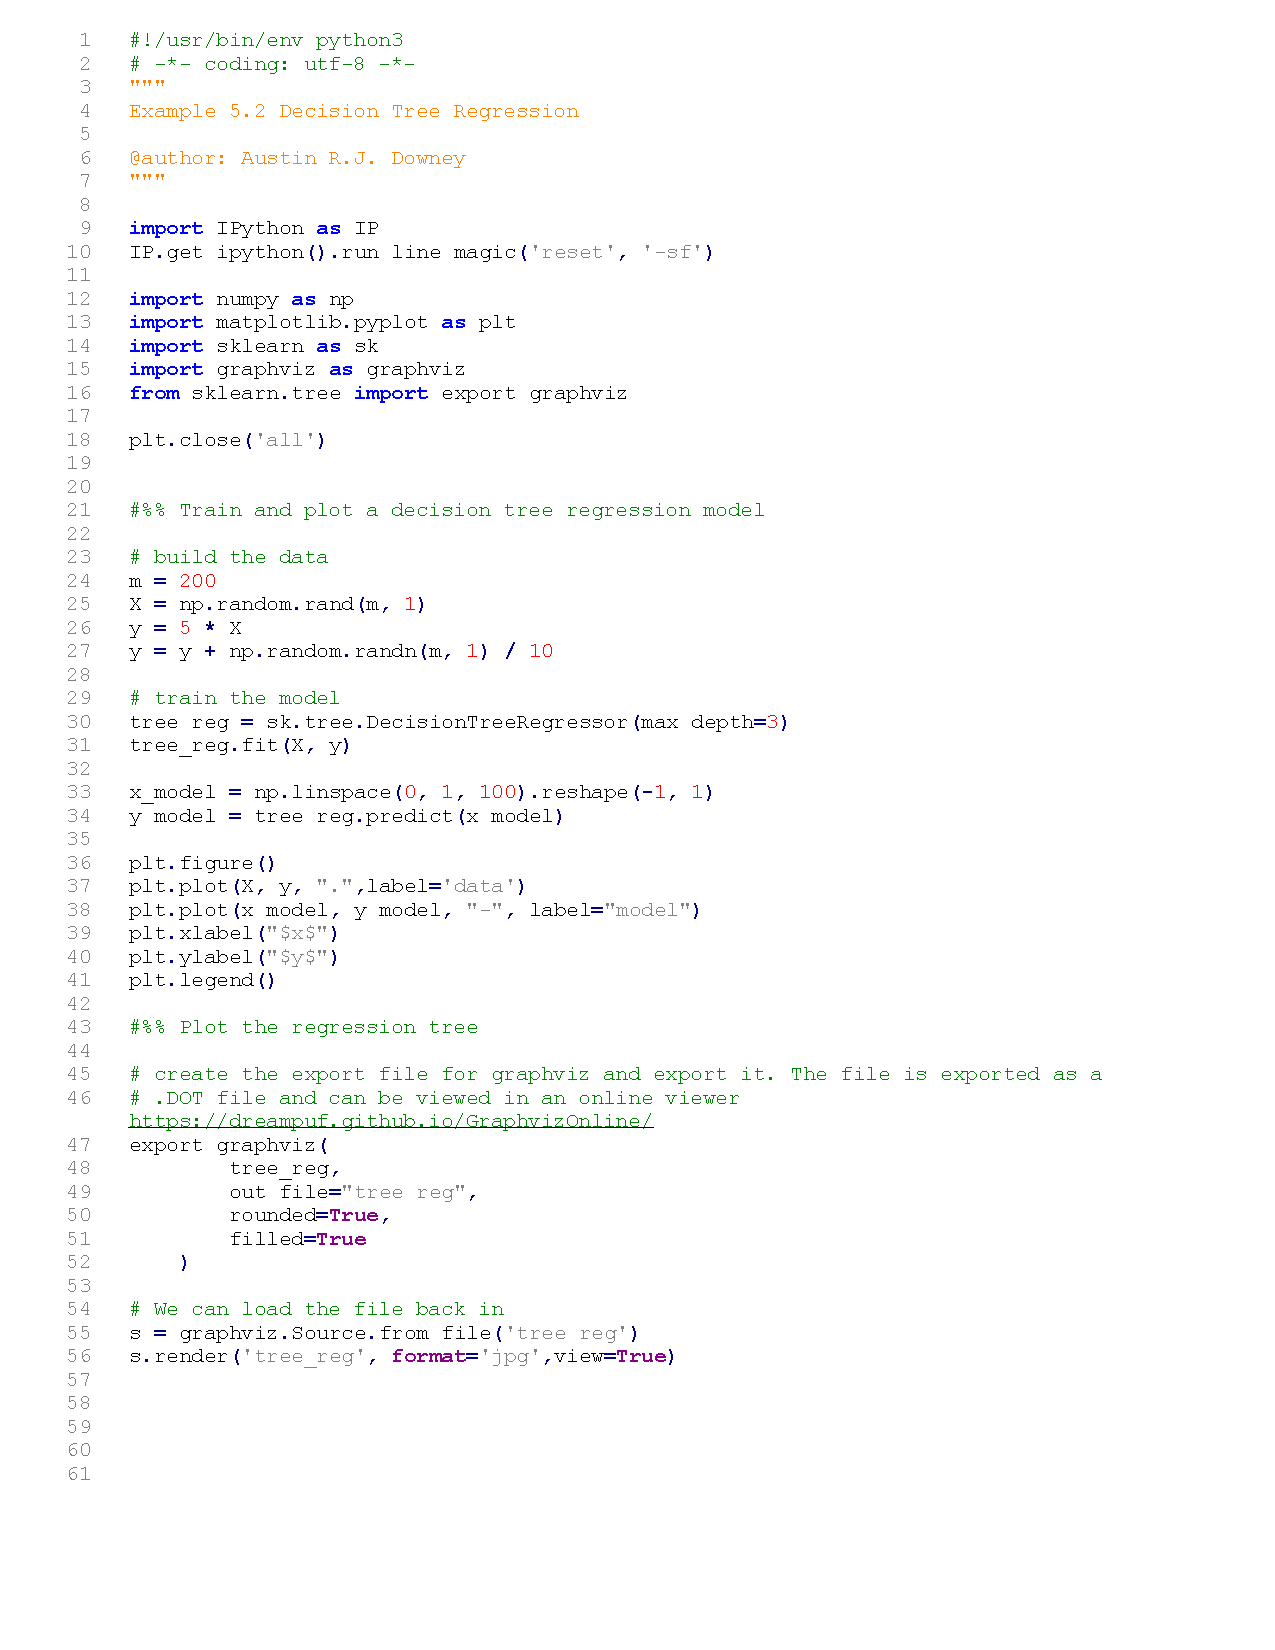
\includepdf[pages=-, width= 0.95\textwidth, pagecommand = {\subsubsection*{Example 5.2}\vspace{0.5em}}]{../code/example_5.2_DecisionTree_regression.pdf}



\end{document}

